\documentclass[a4paper, 12pt]{article}

\usepackage[utf8]{inputenc}
\usepackage[spanish]{babel}
\usepackage[margin=1.5in]{geometry}
\usepackage{graphicx}
\usepackage{float}
\usepackage{pdfpages}
\usepackage{listings}
\usepackage{listingsutf8}
\usepackage{xcolor}
\usepackage{scrextend}
\usepackage{array, multirow}
\usepackage{booktabs}
\usepackage{tabularx}

\definecolor{mGreen}{rgb}{0,0.6,0}
\definecolor{mGray}{rgb}{0.5,0.5,0.5}
\definecolor{mPurple}{rgb}{0.58,0,0.82}
\definecolor{backgroundColour}{rgb}{0.95,0.95,0.92}

\newcolumntype{C}[1]{>{\centering\arraybackslash}p{#1}}

\lstset{
language=C,
%backgroundcolor=\color{backgroundColour},   
commentstyle=\color{mGreen},
%keywordstyle=\color{magenta},
keywordstyle=\color{blue},
%numberstyle=\tiny\color{mGray},
stringstyle=\color{mPurple},
tabsize=4,
basicstyle=\fontsize{11}{13}\ttfamily\footnotesize,
showspaces=false,
showstringspaces=false,
captionpos=b,
breaklines=true
}

%\lstdefinestyle{CStyle}{
%    backgroundcolor=\color{backgroundColour},   
%    commentstyle=\color{mGreen},
%    keywordstyle=\color{magenta},
%    numberstyle=\tiny\color{mGray},
%    stringstyle=\color{mPurple},
%    basicstyle=\footnotesize,
%    breakatwhitespace=false,         
%    breaklines=true,                 
%    captionpos=b,                    
%    keepspaces=true,                 
%    numbers=left,                    
%    numbersep=5pt,                  
%    showspaces=false,                
%    showstringspaces=false,
%    showtabs=false,                  
%    tabsize=2,
%    language=C
%}

\title{		\textbf{Trabajo Práctico 3}\\
			\textbf{Data path y pipeline}
			}
			
\author{	Lucas Medrano, \textit{Padrón Nro. 99247}                     	\\
            \texttt{ lucasmedrano97@gmail.com }                           		\\
            Federico Álvarez, \textit{Padrón Nro. 99266}                 	\\
            \texttt{ fede.alvarez1997@gmail.com }                                 	\\[2.5ex]
            \normalsize{Grupo Nro. \quad - 2do. Cuatrimestre de 2018}      	\\
            \normalsize{66.20 Organización de Computadoras}               	\\
            \normalsize{Facultad de Ingeniería, Universidad de Buenos Aires}\\
       }
\date{}

\begin{document}
	\lstset{inputencoding=utf8/latin1} % Incorpora acentos en los listings
	\maketitle
	\thispagestyle{empty}
	\begin{abstract}
		El objetivo de este trabajo es implementar algunas instrucciones en dos configuraciones de una CPU en un emulador de MIPS32: CPU uniciclo, y CPU pipeline.
		Para implementar las instrucciones se deberá modificar tanto el set de instrucciones como el datapath de la CPU.  
	\end{abstract}
			
	\pagebreak
	\thispagestyle{empty}
	\tableofcontents
	\newpage
	
	\setcounter{page}{1}
	
	\section{Desarrollo}
	El trabajo se divide en dos partes:
	\begin{enumerate}
    \item Implementar las instrucciones en una CPU uniciclo.
    \item Implementar las instrucciones en una CPU pipeline.
	\end{enumerate}
	Las instrucciones que se implementaron son las siguientes:
	\begin{enumerate}
    \item andi Rs, Rt, Imm (And immediate). Esta instrucción de tipo I carga en Rs el resultado
de hacer un AND entre el contenido del registro Rt y el valor de 16 bits Imm.
    \item j Rs, Rt (Jump Rs+Rt). Esta instrucción de tipo I carga en el PC el resultado de sumar
los contenidos de los registros Rs y Rt.
	\item lw Rs, Rd*shamt(Rt). Esta instrucción de tipo R carga en el registro Rs la palabra de 32 bits
cuya dirección es Rt + Rd * shamt. Esta última sólo se implementara en la cpu uniciclo.
	\end{enumerate}
	
	\subsection{Implementación}
	\subsubsection{Programa}
	Para realizar el tp se usó el emulador DrMIPS, el cual permite visualizar el datapath que se usa, escribir programas, y seguir tanto el recorrido del programa y las señales en el datapath, como los valores de los registros.
	Modificando los archivos .cpu se modificaron ambos datapaths (unicycle y pipeline), y modificando los archivos .set se adecuaron ambos set de instrucciones para poder implementar las nuevas instrucciones.	
	
	\subsubsection{andi - CPU uniciclo}
	Para esta instrucción no hizo falta agregar ninguna estructura nueva al datapath. Generando un nuevo codigo de operacion (op) y seteando las señales de control de la Unidad de Control y de la ALU  se pudo obtener el resultado deseado.
	
	\subsubsection{andi - CPU pipeline}
	
	\subsubsection{jregs - CPU uniciclo}
	Para poder implementar esta instrucción no bastaban las estructuras que incluía el datapath uniciclo.
	Se agregó un multiplexor que, mediante una entrada de control, decide si la siguiente direccion de PC es el resultado de la operación de la ALU o es la que indica MuxjUMP (PC+4/branch addres o jump address). Así, se puede setear que se sumen los registros indicados por parámetro, y que la siguiente direccion del PC sea dicha suma.
	\subsubsection{jregs - CPU pipeline}
	
	\subsubsection{lw - CPU uniciclo}
	
	\subsection{Datapaths}
	Los datapath utilizados, y modificados, para el trabajo quedaron de la siguiente manera.
	\subsubsection{CPU uniciclo}
	AGREGAR FOTO
	\subsubsection{CPU pipeline}
	AGREGAR FOTO
	\subsection{Pruebas}
	Para cada instrucción implementada se agregan una, o más, pruebas para asegurarse que el comportamiento sea el esperado. Se adjuntan dichas pruebas a los archivos del trabajo.
	
	
	\section{Conclusiones}
	
	\newpage
	\section{Apéndice}
	\subsection{Enunciado}

	\begin{figure}[H]
		\centering
		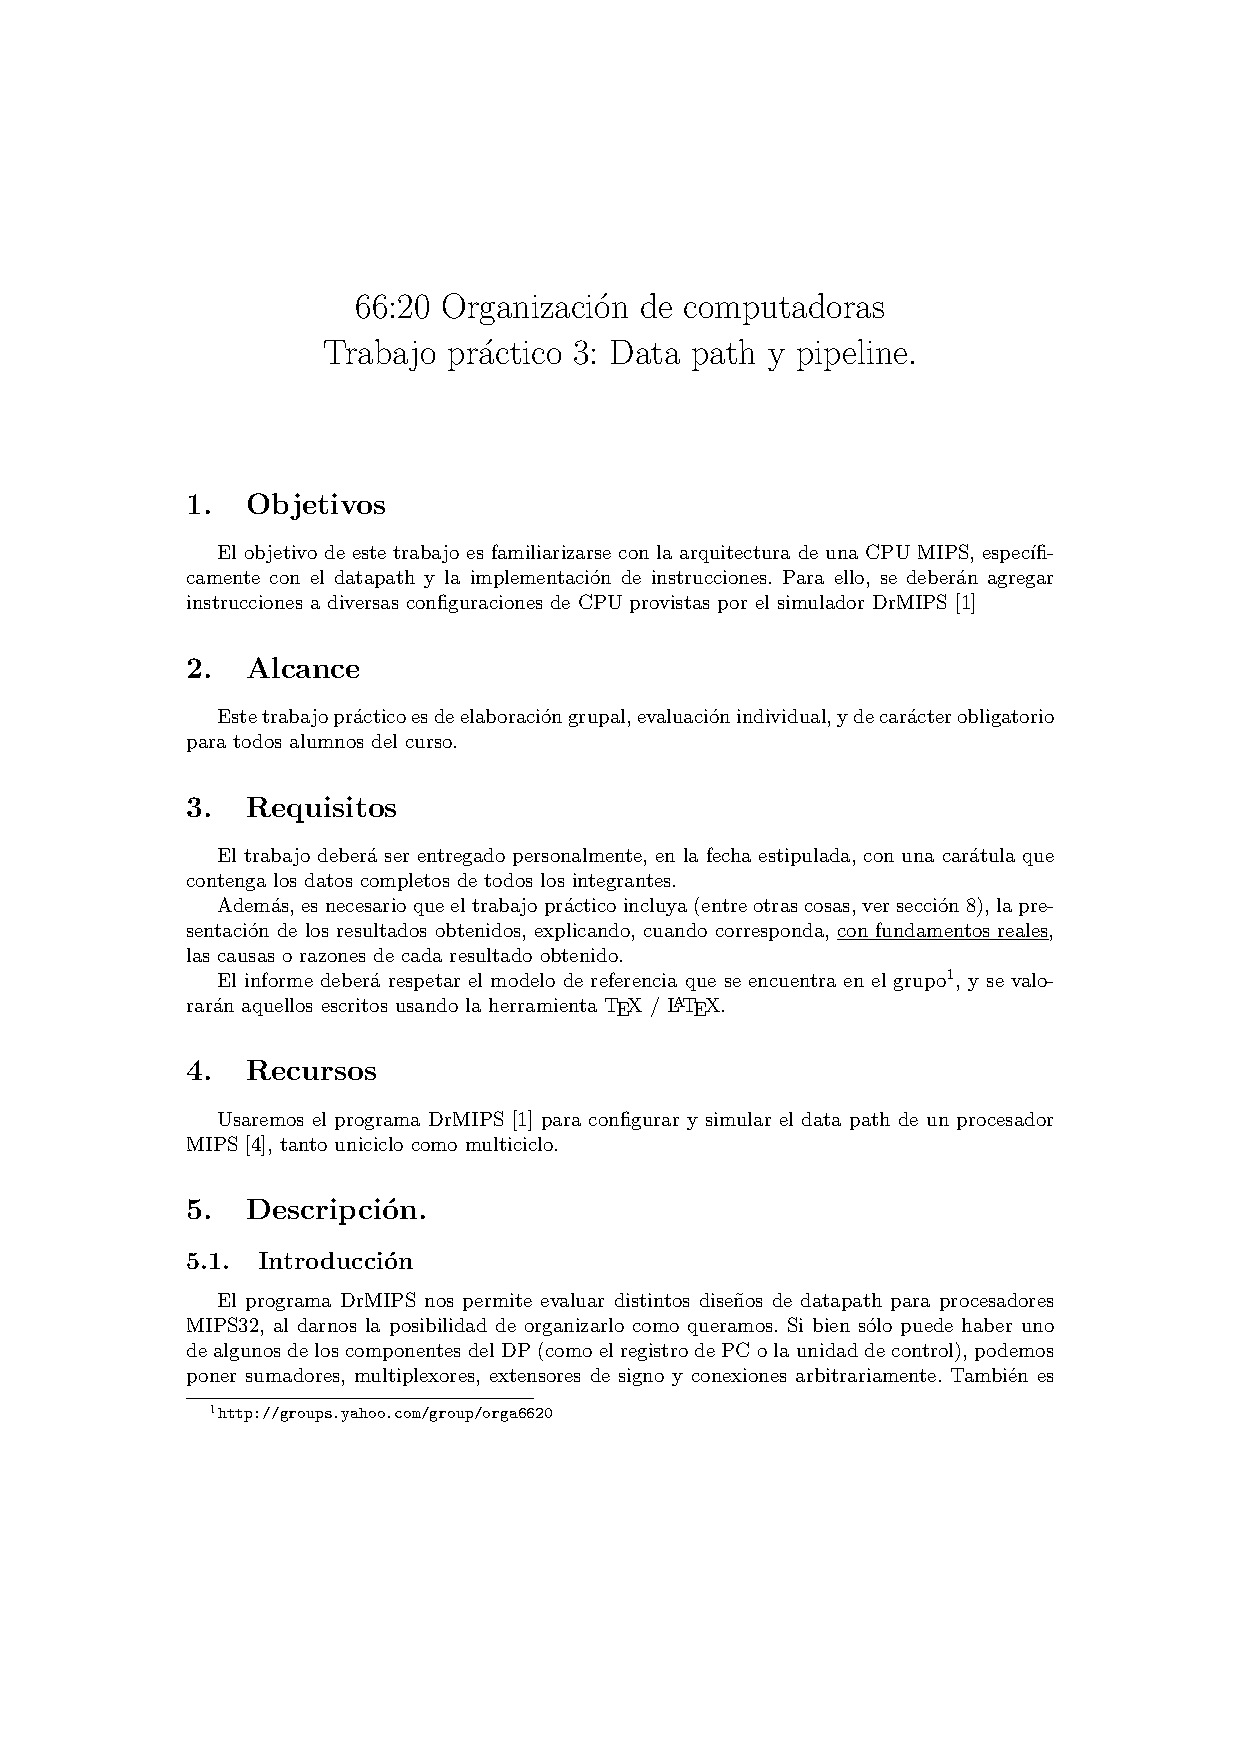
\includegraphics[scale=1, page = 1, clip, trim=1.5in 1.5in 20mm 2in]{files/tp3-c2-2018.pdf}
	\end{figure}
	
	\newpage
	\begin{figure}[H]
		\centering
		\includegraphics[scale=1, page = 2, clip, trim=1.5in 36mm 20mm 1.5in]{files/tp3-c2-2018.pdf}
	\end{figure}
	
	\newpage
	\begin{figure}[H]
		\centering
		\includegraphics[scale=1, page = 3, clip, trim=1.5in 36mm 20mm 1.5in]{files/tp3-c2-2018.pdf}
	\end{figure}
	
	\newpage
	\begin{figure}[H]
		\centering
		\includegraphics[scale=1, page = 4, clip, trim=1.5in 36mm 20mm 1.5in]{files/tp3-c2-2018.pdf}
	\end{figure}
	
\end{document}
